\section{Results}
\label{sec:results}

We report results by hypothesis.
\Tabref{tab:verdicts} gives an overview: the direction of every predicted effect holds, but none of the predicted magnitudes or thresholds matches the data.

\begin{table}[t]
    \centering
    \caption{Summary of hypotheses and verdicts. ``pp'' denotes percentage points; relative changes are with respect to the reference condition.}
    \label{tab:verdicts}
    \small
    \resizebox{\textwidth}{!}{%
    \begin{tabular}{@{}lp{4.1cm}p{5.6cm}l@{}}
        \toprule
        & \textbf{Predicted} & \textbf{Observed} & \textbf{Verdict} \\
        \midrule
        H1 & $-$2 to $-$5\% per doubling beyond 500 tokens & $-$7.7\pp [7.1, 8.3] $\approx -15\%$ relative per doubling & direction holds; 3--6$\times$ larger \\
        H2 & first/last 20\% followed 15--25\% more than middle & lists: ratio 1.04, primacy only; long interleaved prompts: ratio 1.25--1.36 & partly supported \\
        H3 & conflict lowers both rules by 20--30\% & $-$30\% to $-$83\% relative; many ``neither'' outcomes & direction holds; 1.5--3$\times$ larger \\
        H4 & $<$3B saturate at 10 rules; 7B+ hold to 20 & no knee; decline from $N{=}5$ in all models; recipe $>$ size & not supported \\
        \bottomrule
    \end{tabular}}
\end{table}

%-------------------------------------------------------------------
\subsection{Rule count: no saturation point (H4)}
\label{sec:count}

\begin{figure}[t]
    \centering
    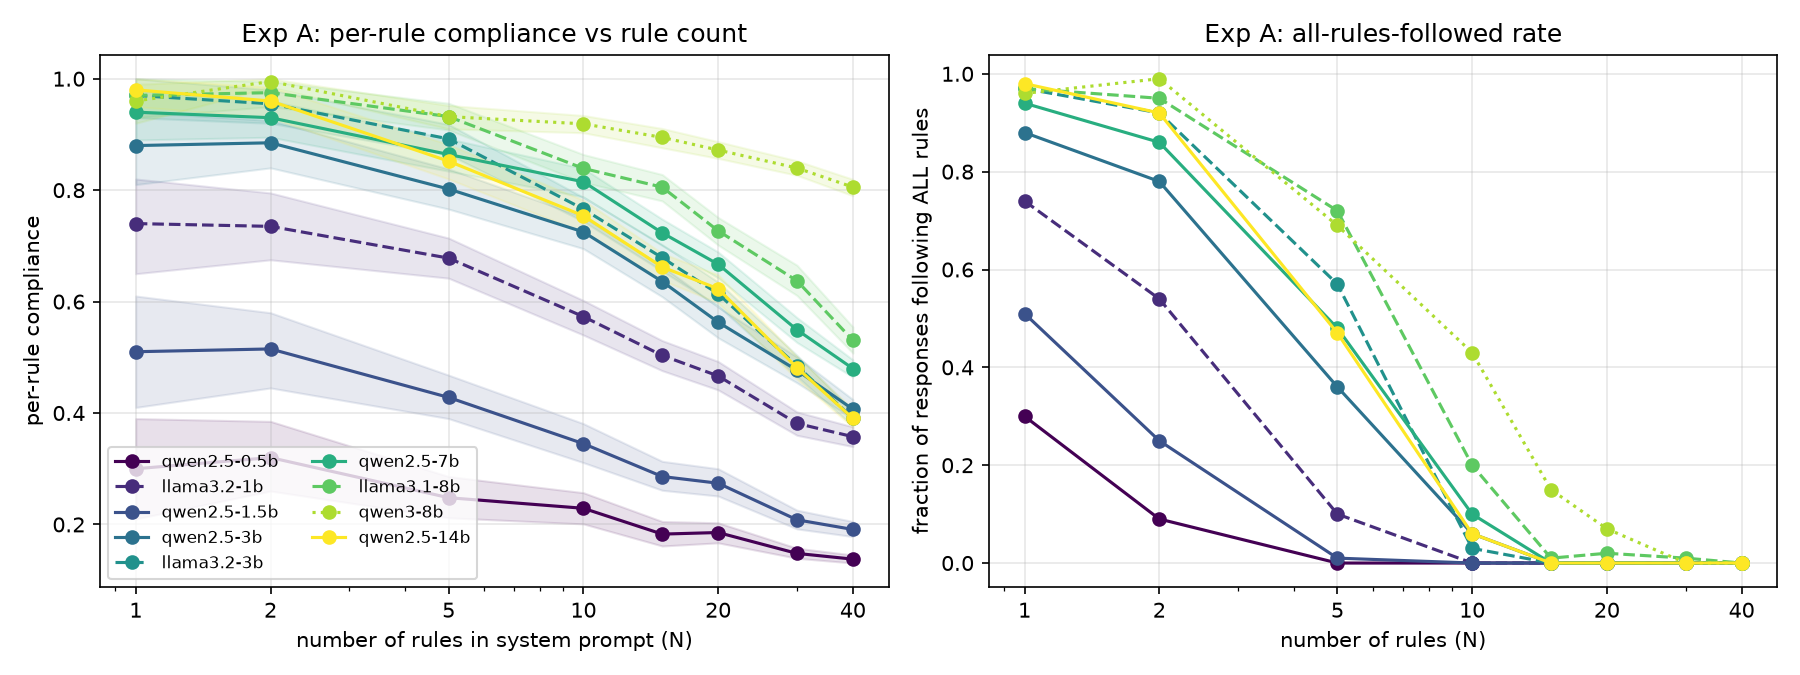
\includegraphics[width=0.95\linewidth]{figures/expA_count.png}
    \caption{\expA: rule count. \figleft Per-rule compliance with item-clustered 95\% bootstrap bands. Every model declines from about five rules onward, with no sharp knee. \qwenthree (dotted) stays near 0.8 even at 40 rules, while \qfourteen (yellow) tracks the 3B models. \figright The fraction of responses that follow {\em all} rules collapses to near zero by $N{=}15$ for every model except \qwenthree.}
    \label{fig:count}
\end{figure}

\begin{table}[t]
    \centering
    \caption{\expA: per-rule compliance (top) and chance-corrected retention $R(N)$ relative to $N{=}1$--2 (bottom). ``First $N$ $<$90\%'' is the smallest rule count at which retention falls below 0.9. Best value in each row in \textbf{bold}.}
    \label{tab:count}
    \resizebox{\textwidth}{!}{%
    \begin{tabular}{@{}lccccccccc@{}}
        \toprule
        & \multicolumn{5}{c}{\textbf{$<$7B}} & \multicolumn{4}{c}{\textbf{$\ge$7B}} \\
        \cmidrule(lr){2-6} \cmidrule(lr){7-10}
        & \textsc{Q-0.5B} & \textsc{L-1B} & \textsc{Q-1.5B} & \textsc{Q-3B} & \textsc{L-3B} & \textsc{Q-7B} & \textsc{L-8B} & \textsc{Qwen3-8B} & \textsc{Q-14B} \\
        \midrule
        \multicolumn{10}{@{}l}{\em Per-rule compliance} \\
        $N{=}1$  & .30 & .74 & .51 & .88 & .97 & .94 & .97 & .96 & \textbf{.98} \\
        $N{=}5$  & .25 & .68 & .43 & .80 & .89 & .86 & \textbf{.93} & \textbf{.93} & .85 \\
        $N{=}10$ & .23 & .57 & .35 & .73 & .77 & .82 & .84 & \textbf{.92} & .75 \\
        $N{=}20$ & .19 & .47 & .27 & .56 & .61 & .67 & .73 & \textbf{.87} & .62 \\
        $N{=}40$ & .14 & .36 & .19 & .41 & .39 & .48 & .53 & \textbf{.80} & .39 \\
        \midrule
        \multicolumn{10}{@{}l}{\em Chance-corrected retention $R(N)$} \\
        $N{=}10$ & .59 & .73 & .58 & .79 & .77 & .85 & .84 & \textbf{.93} & .74 \\
        $N{=}20$ & .36 & .56 & .39 & .58 & .59 & .67 & .72 & \textbf{.89} & .60 \\
        $N{=}40$ & .12 & .37 & .19 & .37 & .31 & .43 & .47 & \textbf{.80} & .31 \\
        First $N$ $<$90\% & 5 & 5 & 5 & 5 & 5 & 5 & 10 & \textbf{20} & 5 \\
        \bottomrule
    \end{tabular}}
\end{table}

{\bf Is there a saturation point?}
H4 predicts a knee: small models should hold steady up to about 10 rules and large models up to about 20.
\Figref{fig:count} and \tabref{tab:count} show no such knee.
Per-rule compliance starts to fall at $N{=}5$ for every model and keeps falling roughly log-linearly up to $N{=}40$.
Hinge regressions place the best breakpoint anywhere between 5 and 30 rules, with no consistent pattern across models.
Retention first drops below 90\% at $N{=}5$ for seven of nine models, at $N{=}10$ for \leight, and at $N{=}20$ for \qwenthree.

{\bf Does size help?}
Larger models degrade more slowly on average.
The 7--8B models keep 84--85\% of their chance-corrected single-rule compliance at 10 rules and 67--72\% at 20; the sub-3B models keep 58--73\% at 10 rules and 36--56\% at 20.
But size alone is a poor predictor.
\qfourteen retains only 74\% at 10 rules, below \qthree (79\%) and \qseven (85\%).
\qwenthree is in a class of its own, with 0.92 per-rule compliance at 10 rules and 0.80 at 40 rules, where the next-best model reaches 0.53.
Among models of similar size, the training recipe matters more than the parameter count.

{\bf Is this a length effect in disguise?}
In \expA, count and length grow together.
\expE holds length at about 4k tokens and still finds a decline with $N$ for all six models that ran it (\appref{app:expE}).
For example, from $N{=}5$ to $40$, \leight falls from 0.44 to 0.27 and \lthree from 0.44 to 0.24.
The slope is flatter than in \expA because 4k tokens of padding already push compliance toward the floor.

%-------------------------------------------------------------------
\subsection{Prompt length: a steep, early decline (H1)}
\label{sec:length}

\begin{figure}[t]
    \centering
    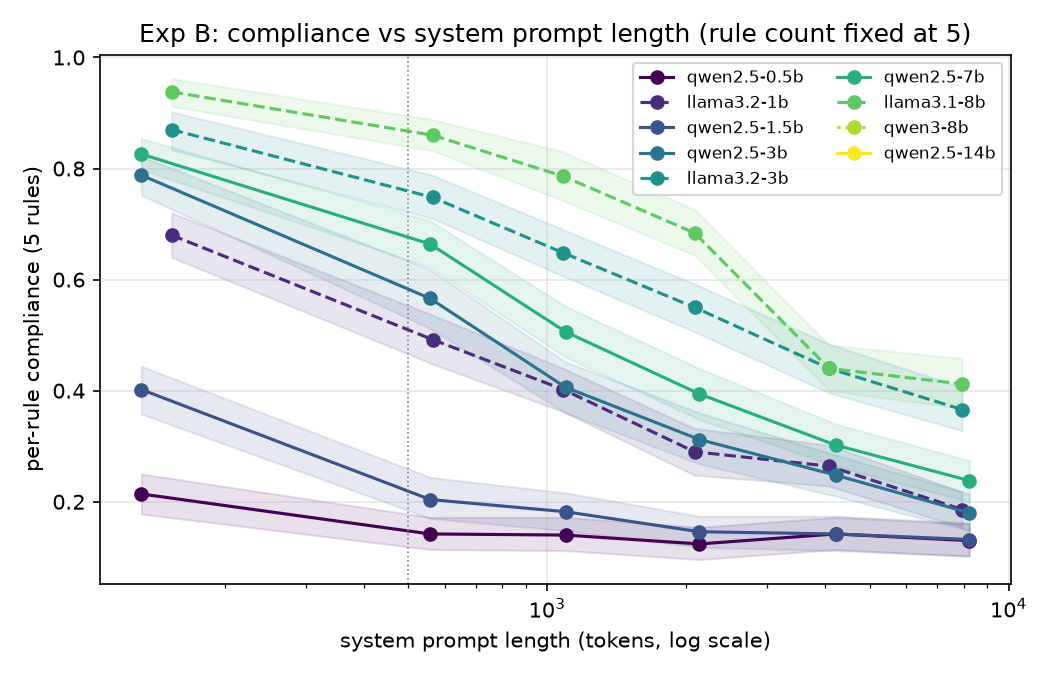
\includegraphics[width=0.62\linewidth]{figures/expB_length.png}
    \caption{\expB: per-rule compliance with five rules as a function of total system-prompt length (log scale; dotted line at 500 tokens). Bands are 95\% bootstrap CIs. Compliance falls steadily with every doubling, and the drop begins before 500 tokens. \qwenthree and \qfourteen did not complete \expB.}
    \label{fig:length}
\end{figure}

\begin{table}[t]
    \centering
    \caption{\expB: per-rule compliance with five interleaved rules as padding grows (left) and the slope per doubling of prompt length for prompts of at least 500 tokens (right; rule fixed effects, item-clustered 95\% CIs, Holm-corrected $p$). The pooled slope is about three to six times the hypothesized 2--5\% per doubling.}
    \label{tab:length}
    \resizebox{\textwidth}{!}{%
    \begin{tabular}{@{}lcccccccccc@{}}
        \toprule
        & \multicolumn{6}{c}{\textbf{Padding (tokens)}} & \multicolumn{3}{c}{\textbf{Slope per doubling}} \\
        \cmidrule(lr){2-7} \cmidrule(lr){8-10}
        \textbf{Model} & 0 & 500 & 1k & 2k & 4k & 8k & pp [95\% CI] & relative & Holm $p$ \\
        \midrule
        \qhalf    & .21 & .14 & .14 & .12 & .14 & .13 & $-$0.6 [$-$1.1, $-$0.1] & $-$4\% & 0.02 \\
        \lone     & .68 & .49 & .40 & .29 & .26 & .19 & $-$8.0 [$-$9.1, $-$6.9] & $-$16\% & $<$1e-30 \\
        \qonefive & .40 & .20 & .18 & .15 & .14 & .13 & $-$2.4 [$-$3.1, $-$1.6] & $-$12\% & $<$1e-9 \\
        \qthree   & .79 & .57 & .41 & .31 & .25 & .18 & $-$10.0 [$-$11.2, $-$8.8] & $-$18\% & $<$1e-50 \\
        \lthree   & .87 & .75 & .65 & .55 & \textbf{.44} & .37 & $-$9.7 [$-$10.9, $-$8.5] & $-$13\% & $<$1e-50 \\
        \qseven   & .83 & .66 & .51 & .39 & .30 & .24 & $-$11.0 [$-$12.0, $-$9.9] & $-$17\% & $<$1e-80 \\
        \leight   & \textbf{.94} & \textbf{.86} & \textbf{.79} & \textbf{.68} & \textbf{.44} & \textbf{.41} & $-$12.5 [$-$13.7, $-$11.4] & $-$15\% & $<$1e-90 \\
        \midrule
        Pooled (7 models) & & & & & & & $-$7.7 [$-$8.3, $-$7.1] & $-$15\% & 2e-149 \\
        \bottomrule
    \end{tabular}}
\end{table}

{\bf How fast does compliance fall with length?}
\Figref{fig:length} and \tabref{tab:length} show the result of holding the rule count at five and adding neutral padding.
Pooled over seven models, per-rule compliance falls by 7.7\pp per doubling beyond 500 tokens (95\% CI 7.1--8.3), about 15\% in relative terms.
H1 predicted 2--5\%, so the direction holds but the effect is three to six times larger.
For models that are competent at short lengths, the slope is 8--12.5\pp per doubling.
\qseven goes from 0.83 with no padding to 0.24 at about 8k tokens, and \qthree from 0.79 to 0.18.

{\bf When does the decline start?}
The decline begins well before 500 tokens.
Adding the first 500 tokens of padding costs 8--22\pp in competent models.
The two smallest Qwen models have small slopes only because they are already near their base rates without padding.

%-------------------------------------------------------------------
\subsection{Position: primacy in lists, recency in long prompts (H2)}
\label{sec:position}

\begin{figure}[t]
    \centering
    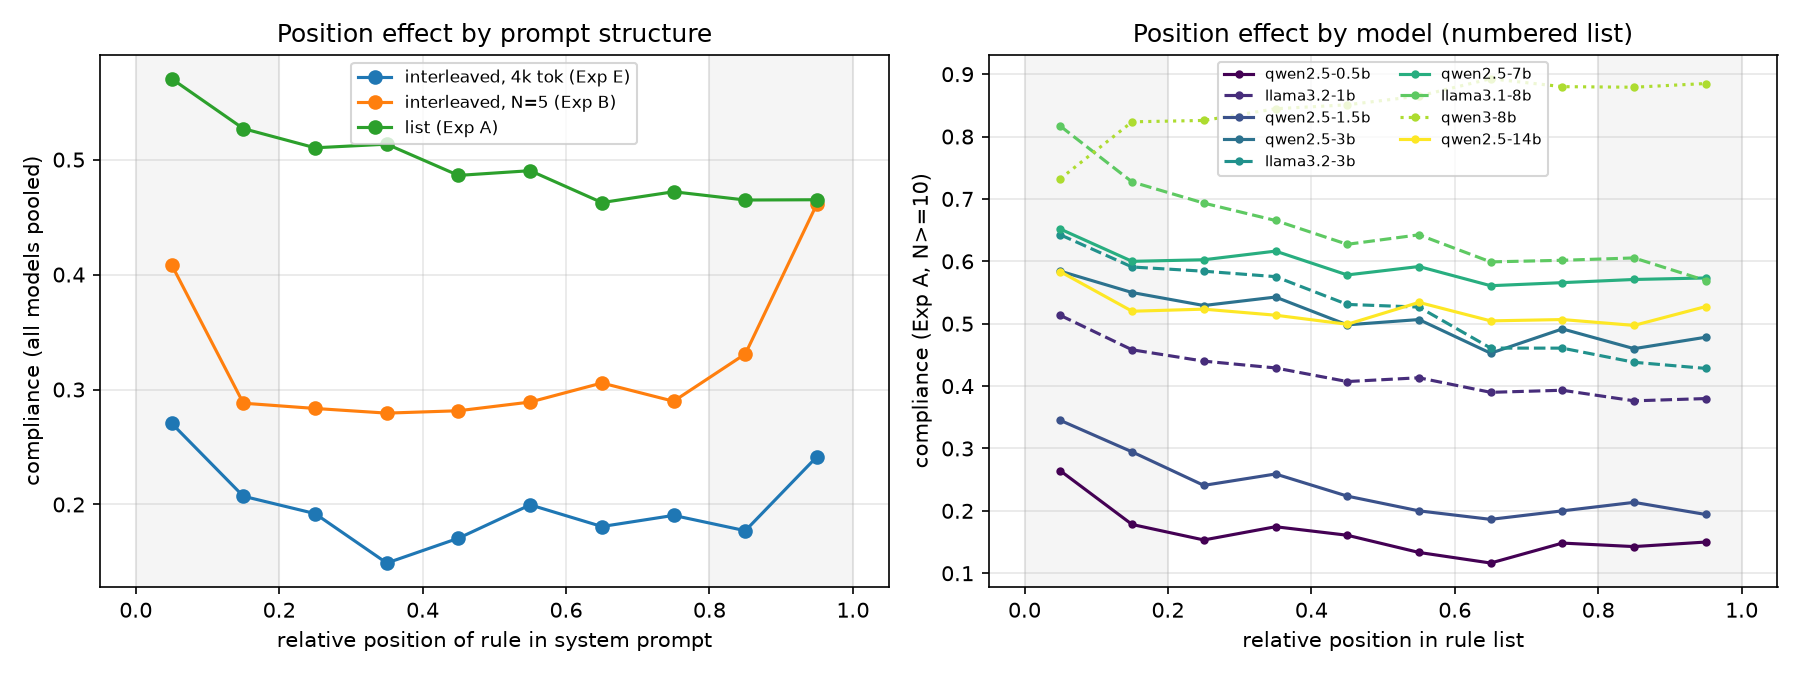
\includegraphics[width=0.95\linewidth]{figures/position.png}
    \caption{Compliance by relative rule position (deciles; shaded regions mark the first and last 20\%). \figleft Pooled over models. Rules in a short numbered list (\expA, green) show mild primacy and no end advantage. Rules interleaved in long padding (\expB, orange; \expE, blue) show a U-shape with the strongest effect at the end. \figright Per-model curves for numbered lists with $N \ge 10$. Most models favor early rules; \qwenthree (dotted) is the exception and favors late rules.}
    \label{fig:position}
\end{figure}

\begin{table}[t]
    \centering
    \caption{Compliance by rule position, pooled over models with rule and condition fixed effects. The ratio compares the mean of the two edge bins to the middle (95\% bootstrap CI). Differences are fixed-effect estimates; *** $p < 0.001$. H2 predicts a ratio of 1.15--1.25.}
    \label{tab:position}
    \resizebox{\textwidth}{!}{%
    \begin{tabular}{@{}lcccccc@{}}
        \toprule
        \textbf{Structure} & \textbf{First 20\%} & \textbf{Middle} & \textbf{Last 20\%} & \textbf{Edge / middle} & \textbf{First vs.\ mid} & \textbf{Last vs.\ mid} \\
        \midrule
        Numbered list (\expA, $N \ge 10$)          & \textbf{.550} & .489 & .465 & 1.04 [1.02, 1.06] & +5.0\pp*** & $-$2.8\pp*** \\
        Interleaved, $N{=}5$ (\expB, $\ge$1k tokens) & .365 & .287 & \textbf{.412} & \textbf{1.36} [1.23, 1.49] & +7.1\pp*** & +9.4\pp*** \\
        Interleaved, $\sim$4k tokens (\expE)       & \textbf{.239} & .180 & .212 & 1.25 [1.15, 1.35] & +6.0\pp*** & +4.9\pp*** \\
        \bottomrule
    \end{tabular}}
\end{table}

{\bf Are rules at the edges followed more often?}
The answer depends on how the rules are laid out (\tabref{tab:position}, \figref{fig:position}).
In a plain numbered list, the first 20\% of rules gain 5.0\pp (about 10\% relative) over the middle, but the last 20\% lose 2.8\pp.
The edge-to-middle ratio is only 1.04, far below the predicted 1.15--1.25.
When rules are scattered through long padding, both edges gain and the end gains most: the ratio is 1.36 for \expB and 1.25 for \expE, which meets or exceeds the prediction.

{\bf Do models agree?}
In numbered lists, 8 of 9 models favor early rules: the first 20\% gain 3 to 13\pp and the last 20\% lose 0 to 9\pp.
\leight shows the strongest primacy (+12.8\pp for the first 20\%, $-$5.2\pp for the last 20\%), and \lthree shows a similar pattern (+8.7\pp, $-$9.3\pp).
\qwenthree is the reverse: its first 20\% lose 8.7\pp and its last 20\% gain 2.1\pp.

%-------------------------------------------------------------------
\subsection{Block placement: the end of the prompt wins}
\label{sec:placement}

\begin{figure}[t]
    \centering
    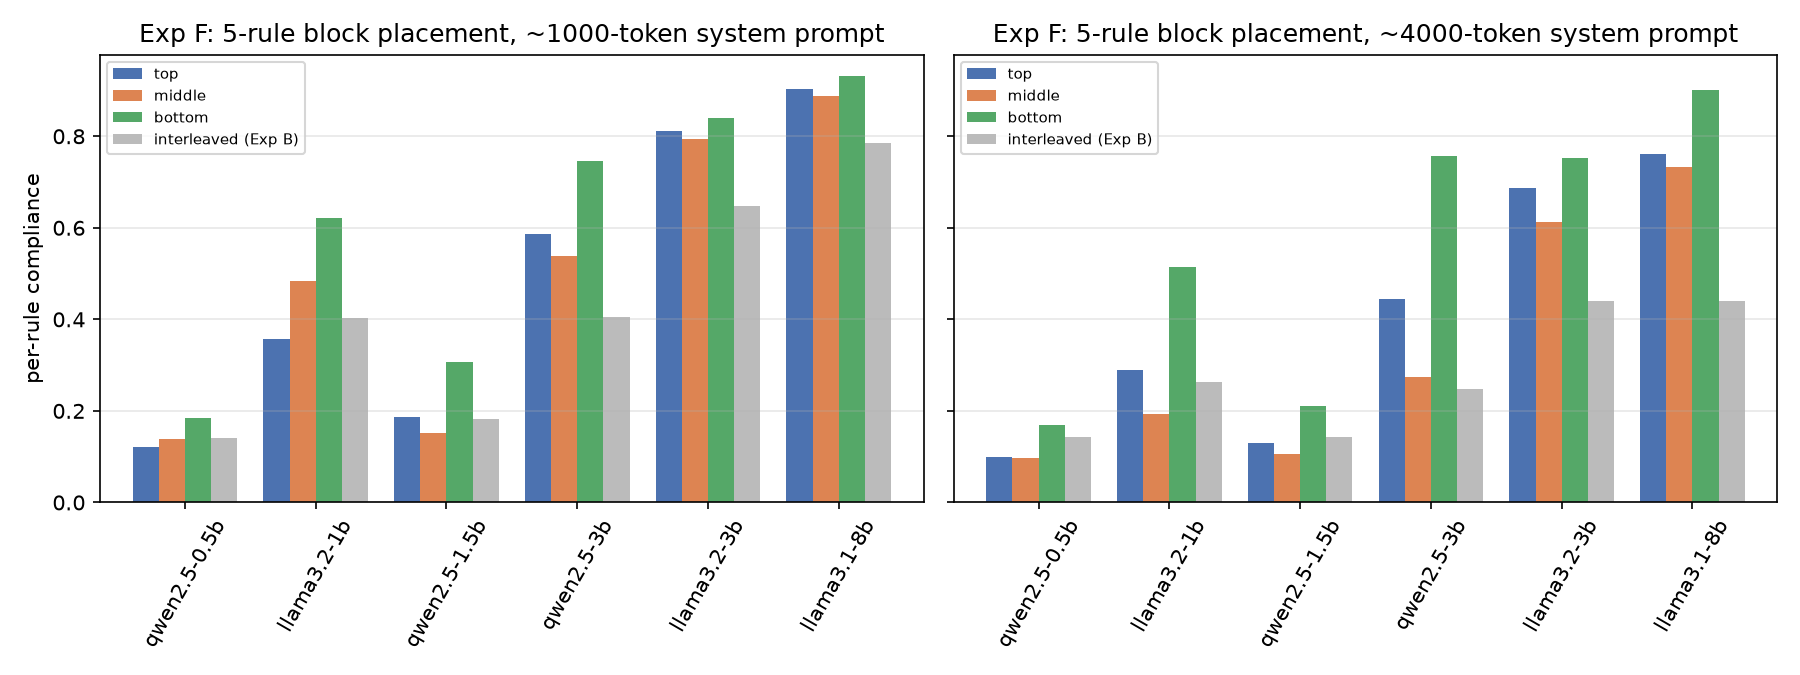
\includegraphics[width=0.95\linewidth]{figures/expF_placement.png}
    \caption{\expF: the same five rules as one numbered block placed at the top, middle, or bottom of a $\sim$1k-token \figleft or $\sim$4k-token \figright system prompt. Grey bars show the same rules interleaved through the padding (\expB). A block at the bottom, right before the user turn, is best for every model; at 4k tokens it recovers most of the loss for \qthree and \leight.}
    \label{fig:placement}
\end{figure}

\begin{table}[t]
    \centering
    \caption{\expF: per-rule compliance for a five-rule block at different positions, pooled over six models (left), and pooled placement effects relative to the middle with rule and model fixed effects (right; 95\% CIs). Best placement in \textbf{bold}.}
    \label{tab:placement}
    \small
    \begin{tabular}{@{}lccccccc@{}}
        \toprule
        & \multicolumn{4}{c}{\textbf{Compliance}} & \multicolumn{2}{c}{\textbf{Effect vs.\ middle}} \\
        \cmidrule(lr){2-5} \cmidrule(lr){6-7}
        \textbf{Length} & Interleaved & Top & Middle & Bottom & Top & Bottom \\
        \midrule
        $\sim$1k tokens & .43 & .49 & .50 & \textbf{.61} & +1.7\pp ($p{=}0.11$) & \textbf{+11.0\pp} [8.9, 13.1] \\
        $\sim$4k tokens & .28 & .40 & .34 & \textbf{.55} & +6.3\pp [4.1, 8.4] & \textbf{+20.8\pp} [18.6, 23.0] \\
        \bottomrule
    \end{tabular}
\end{table}

{\bf Why does length hurt?}
\expB mixes two possible causes: rules move farther from the end of the prompt, and rules are scattered among unrelated text.
\expF separates them by keeping the five rules together in one block and moving only the block (\figref{fig:placement}, \tabref{tab:placement}).
At about 4k tokens, the pooled compliance is 0.55 for a block at the bottom, 0.40 at the top, 0.34 in the middle, and 0.28 for the same rules interleaved.
A bottom block beats a middle block by 11.0\pp at 1k tokens and by 20.8\pp at 4k tokens.
Both causes therefore matter: distance from the end of the prompt is the larger factor, and a contiguous block beats scattered rules at every placement.

The effect is large for individual models.
\qthree reaches 0.76 with a bottom block at 4k tokens, close to its no-padding score of 0.80, compared with 0.27 in the middle and 0.25 when interleaved.
\leight reaches 0.90 at the bottom, 0.73 in the middle, and 0.76 at the top, but only 0.44 when its rules are interleaved.

These findings reconcile the two position patterns in \secref{sec:position}.
In a short list, every rule is close to the end of the prompt, so order within the list matters most and primacy appears.
In a long prompt, distance from the end dominates.

%-------------------------------------------------------------------
\subsection{Conflicting rules: large drops and compromises (H3)}
\label{sec:conflict}

\begin{figure}[t]
    \centering
    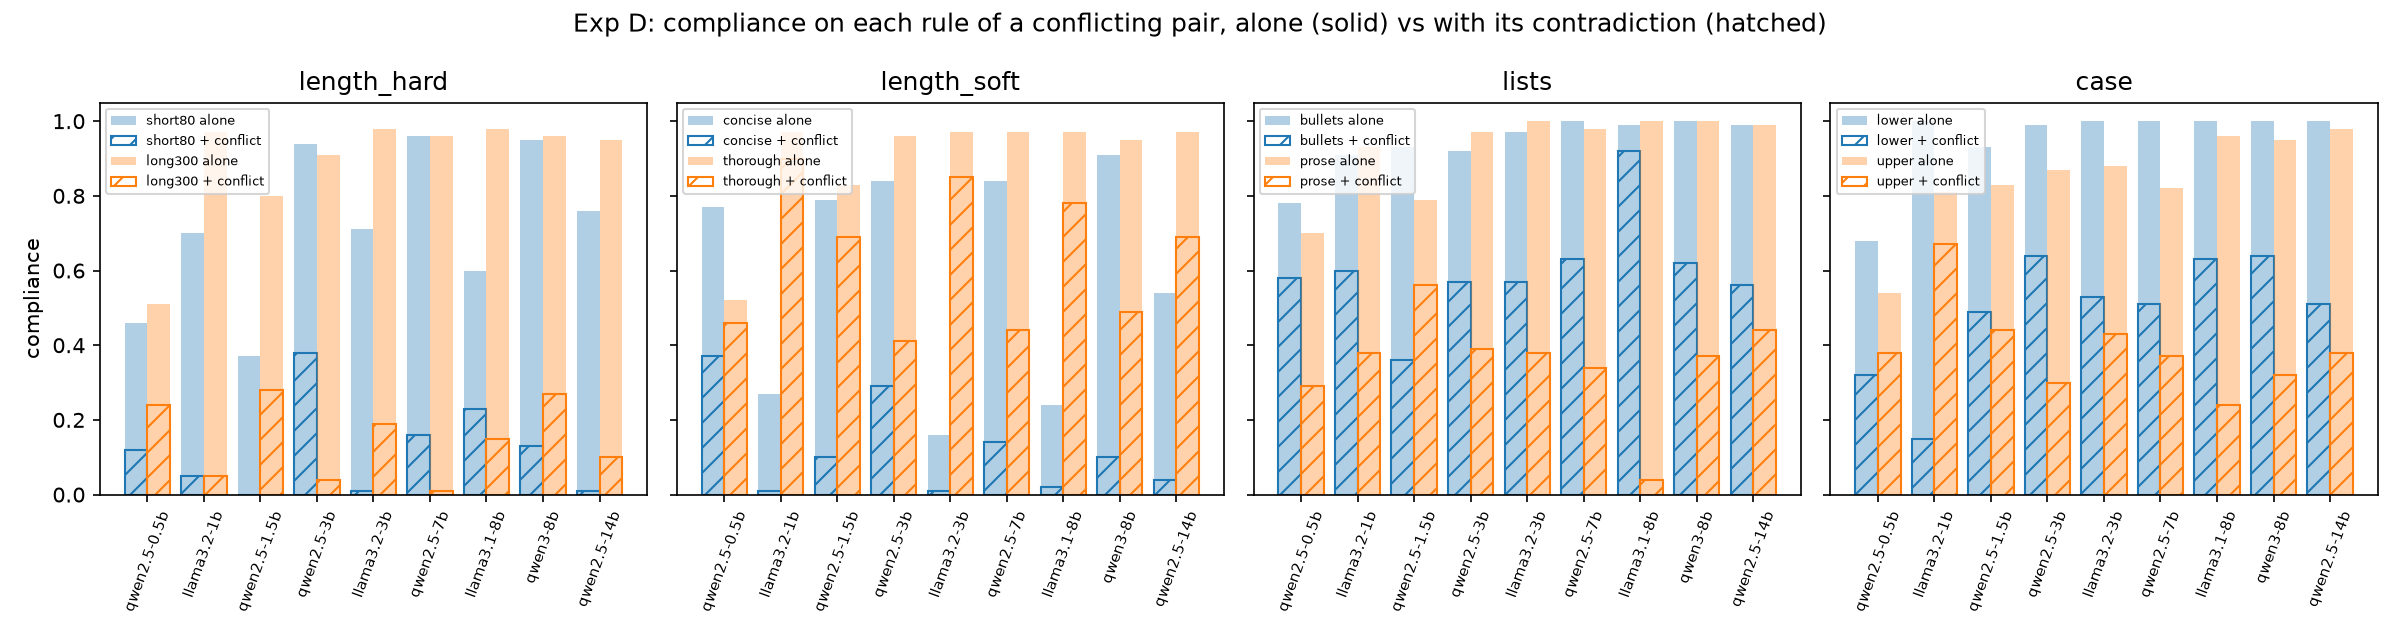
\includegraphics[width=\linewidth]{figures/expD_conflict.png}
    \caption{\expD: compliance with each rule of a contradictory pair when given alone (solid) and together with its contradiction (hatched), per model. For the length pairs, both hatched bars are often low at once, because responses settle on an intermediate length that satisfies neither rule. For \textsc{length\_soft}, the ``thorough'' rule (orange) keeps most of its compliance while ``concise'' collapses.}
    \label{fig:conflict}
\end{figure}

\begin{table}[t]
    \centering
    \caption{\expD: compliance on each member of a conflict pair, alone vs.\ with its contradiction, pooled over 9 models ($n{=}900$ paired items per row). Relative changes with 95\% bootstrap CIs. All rows have McNemar $p<10^{-10}$. The smallest drop is in \textbf{bold}; it is the only one inside the hypothesized 20--30\% band.}
    \label{tab:conflict}
    \small
    \begin{tabular}{@{}llccc@{}}
        \toprule
        \textbf{Pair} & \textbf{Rule} & \textbf{Alone} & \textbf{With contradiction} & \textbf{Relative change} \\
        \midrule
        \multirow{2}{*}{\textsc{length\_hard}} & $<$80 words & .72 & .12 & $-$83\% [$-$87, $-$79] \\
        & $\ge$300 words & .89 & .15 & $-$83\% [$-$87, $-$80] \\
        \midrule
        \multirow{2}{*}{\textsc{length\_soft}} & be concise ($<$150 w) & .60 & .12 & $-$80\% [$-$84, $-$75] \\
        & explain thoroughly ($\ge$250 w) & .90 & .63 & \textbf{$-$30\%} [$-$35, $-$25] \\
        \midrule
        \multirow{2}{*}{\textsc{lists}} & bulleted list & .94 & .60 & $-$36\% [$-$43, $-$29] \\
        & no lists & .93 & .35 & $-$62\% [$-$68, $-$55] \\
        \midrule
        \multirow{2}{*}{\textsc{case}} & all lowercase & .96 & .49 & $-$49\% [$-$53, $-$44] \\
        & ALL UPPERCASE & .85 & .39 & $-$54\% [$-$58, $-$49] \\
        \bottomrule
    \end{tabular}
\end{table}

{\bf How much does a contradiction cost?}
Adding the contradicting rule lowers compliance on each member of a pair by 30--83\% relative (\tabref{tab:conflict}).
Every pooled comparison has $p < 10^{-10}$, and 66 of the 72 per-model tests stay significant after Holm correction.
H3 predicted 20--30\%, so the direction holds but the drop is 1.5--3 times larger.
Because the rules in each pair are mutually exclusive, a large drop is expected; the more informative question is how models resolve the conflict.

{\bf How do models resolve conflicts?}
For length conflicts, models usually compromise and satisfy neither rule.
With ``fewer than 80 words'' plus ``at least 300 words'', 58\% (\qthree) to 90\% (\lone) of responses meet neither constraint.
The median length with both rules is 96--220 words, compared with about 50--90 words for the short rule alone and about 350--500 words for the long rule alone.
For format and case conflicts, one rule usually wins: ``neither'' outcomes are only 0--13\% for 8 of 9 models.
The winner is stable within a model (\eg \leight chooses bullets 92\% of the time), and it is not simply the rule that appears later, since rule order was randomized.

{\bf Is the soft conflict symmetric?}
No.
Every model leans toward ``explain thoroughly'': ``be concise'' loses 80\% of its compliance, while ``explain thoroughly'' loses only 30\%.
This is the only result inside the hypothesized 20--30\% band.

{\bf Do conflicts hurt other rules?}
Barely.
Background keyword rules move by only 0--8\pp between conflict and no-conflict conditions, with no consistent sign.
The cost of a contradiction stays within the contradicting pair.

%-------------------------------------------------------------------
\subsection{Qualitative analysis and reproducibility}
\label{sec:qualitative}

\para{Rules are silently dropped.}
At 8k tokens, \qseven writes well-formed, on-topic answers that ignore most rules.
It is not confused by the padding; it behaves as if the rules were not there.
Rules that responses often satisfy naturally survive (bold text, numbered lists, exclusions), while arbitrary keywords such as ``velvet'', ``pineapple'', ``consequently'', and ``indeed'' twice fall to nearly zero at 4--8k tokens.

\para{Compromises can be strange.}
Given ``fewer than 80 words'' and ``at least 300 words'', \qseven wrote 143 words.
Given ``all lowercase'' and ``all UPPERCASE'' together with a rule to include ``gracias'', it wrote its name ``orion'' in lowercase and then switched to an all-caps answer in Spanish.
Satisfying one rule spilled over into an odd reading of another.

\para{Exclusion rules carry little signal.}
Rules such as ``never use {\em really}'' have base rates of 81--99\%, so they look followed regardless of condition.
The headline effects come from inclusion and format rules, and the retention metric corrects for this.

\para{Reproducibility.}
We re-ran \qonefive on all of \expA (900 prompts, 12{,}300 rule checks) in a separate process on a different GPU with a different KV-cache size.
Because vLLM greedy decoding is not batch-invariant, only 13\% of responses were byte-identical.
Even so, 93.7\% of individual rule checks agreed, and mean compliance changed by only 0.07\pp (0.2503 vs.\ 0.2496).
Aggregate effects are therefore stable under decoding noise, even though single responses are not deterministic.
